% !TEX root = ../Thesis.tex
\begin{document}
\documentclass[Thesis.tex]{subfiles}
\chapter{Fine-grained information presentation}
\label{ch:infpres}



%To be able to show or hide specific parts of the letters we try to break them apart into useful sections. (Irgendwie kein runder Übergang. Bin mir auch nicht ganz sicher, ob der nächste Teil noch in die Intro gehört. Macht aber schon Sinn, dann kann ich im nächsten Kapitel gleich mit einer Anwendung anfangen, für die ich alle anderen Methoden einführen muss.)
Many physician letters are rather long documents, spanning several pages. To increase the usability of a recommender system used in practice it is desirable to be able to show specific information like the diagnosis or the therapy history on demand or hide unnecessary parts of the letters like the introduction. It might also be desirable to compare letters only based on a specific section like therapy history. A first step towards this goal is the automatic extraction of the relevant paragraphs.



\section{Paragraph Extraction}

%As already mentioned above, the letters almost always contain separate
%paragraphs like greeting, diagnosis, therapy history and anamnesis.
%To be able to hide unnecessary information or to only present requested
%information it is useful to automatically extract individual
%paragraphs from the documents. 
The XML data format of the letters allows to automatize inspection of rather fine-grained structures present in the letters. One can automatically determine boldfaced characters for example. Because of this and because the documents are similar in structure, we use a rule based approach for extracting
the individual paragraphs. A simplified rule to find the beginning of the diagnosis paragraph is shown in pseudocode:
%\bigskip
%
%\begin{algorithm}[H]
%	\DontPrintSemicolon
%	diagnosisRegex = '[dD]iagnose(n)?'\;
%	text = thisXmlNode.text()\;
%	\If{regex.match(text, diagnosisRegex)
%		$ {\bf and} $ boldface(text)
%		$ {\bf and} $ precededByNewline(thisXmlNode)}{
%		diagnosisStart = thisXmlNode\;
%		}
%		
%		\caption{Simplified pseudocode algorithm to find the beginning of the diagnosis paragraph}
%\end{algorithm}
%		
%\bigskip
\bigskip

\begin{lstlisting}
diagnosis_regex = '[dD]iagnose(n)?'
text = this_xml_node.text()
if diagnosis_regex.match(text)
	and boldface(text)
	and preceded_by_newline(this_xml_node):
then:
	diagnosis_start = this_xml_node
\end{lstlisting}

\bigskip
%(Weder der erste noch der zweite pseudocode gefällt mir bis jetzt. Wird noch geändert.)

A regular expression is defined that matches the beginning of the diagnosis paragraph (the German word for diagnosis is "Diagnose").
The text of every node in the XML tree is checked for a regular expression match and several other rules. If an XML node matches all criteria it is marked as the beginning of the diagnosis paragraph.
With a set of rules like the one above we automatically extract the
paragraphs of interest from the documents. This approach, however,
is not completely reliable, as the doctors are free to write the documents
in the way they please. Indeed we find several wrongly extracted paragraphs,
that e.g. include the subsequent paragraph as well. For our dataset
it is possible to check the extraction process by hand. However, this
is tedious work and is not scalable to bigger
datasets. We therefore explore whether we can in principle make use
of other automated methods to find paragraphs for which the extraction
process does not produce desired results. We therefore take several correctly extracted and one incorrectly extracted
diagnosis paragraphs and convert them to their bag of words representation.
To get a feeling for how these vectors behave we use Principle Component
Analysis (PCA) to get a lower dimensional approximation of the vectors. PCA finds the linear
subspace with desired dimensionality of the original space that preserves as much of the variance of the vectors in the original space as possible. Thereby one can gain a low dimensional approximation of the high dimensional data and use this approximation for visual inspection.
See figure \ref{fig:bow_find_odd} for a 2D PCA plot of the bag of words representation
of the correctly and incorrectly extracted diagnosis paragraph. As is apparent from the figure, it would not be a
hard task to automatically detect the outlier. In this case the incorrectly
extracted paragraph includes not only the diagnosis, but also the
therapy history. In cases like this with additional text present, it is an easy task to
identify the incorrect ones. A harder problem arises, when only parts
of the paragraph of interest have been extracted. However, we believe
that this problem is of little concern, due to the way our rules are made.
%The way our rules are built it
%is very unlikely that we will face this problem. The paragraph would
%have to include an empty line, the subsequent one would have to contain
%only boldface characters and a few more conditions would have to be
%fulfilled for this problem to arise.
Indeed, we did not find a case
of this problem in our dataset. (Ich könnte auch mal tatsächliche outlier detection machen, wenn du das für sinnvoll hälst. Hab ein paar Ideen, die gut funktionieren könnten, wollte aber keine Zeit rein stecken, falls wir es nicht benutzen wollen.)
\begin{figure}
	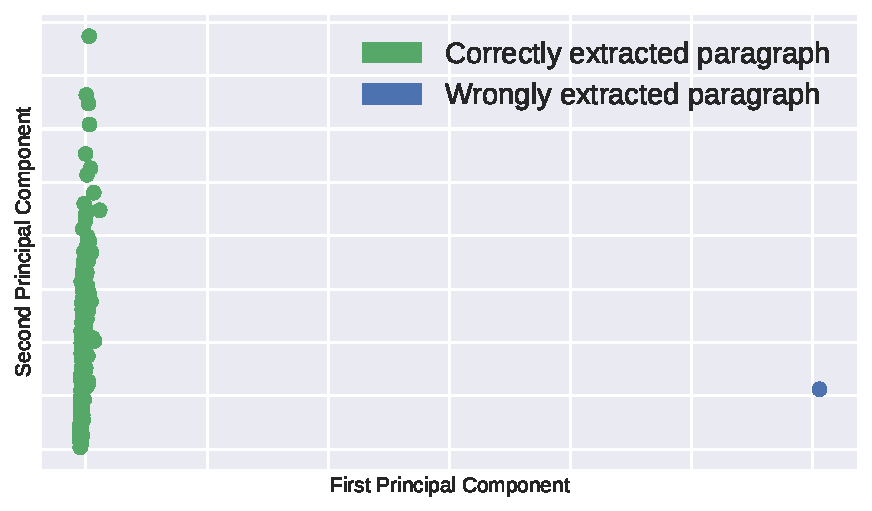
\includegraphics[width=\linewidth]{figures/bow_find_odd}
	\caption{2D PCA projection of bag of words representation of one incorrectly extracted diagnosis paragraph and several correctly extracted ones.}
	\label{fig:bow_find_odd}
\end{figure}




\section{Paragraph Classification}
In our sample dataset, we can automate paragraph extraction as shown above. We can also detect for which paragraphs the procedure produces incorrect results. This approach works well only because the documents in our dataset generally adhere to a rough structure. For datasets from other clinics constructing a rule based extraction procedure is not only time consuming, it might not be possible at all. We therefore test an approach to classification of extracted paragraphs into the respective categories - greeting, diagnosis and anamnesis. Our findings show that surprisingly this is not a hard problem. On unseen datasets it might therefore be possible to split text into unlabeled paragraphs with a basic rule based approach. One can possibly define a new paragraph to begin after a blank line and automatically label the resulting paragraphs with a predefined category. This way one would be able to hide or show specific information on demand even on datasets from other clinics.

We approach the problem again from a vector space based view-point. We first compute the vector representation for every paragraph with different text embedding methods. Then logistic regression is trained on a training portion of the dataset and the performance evaluated on a testing portion. We use leave-one-out cross-validation to obtain a good estimate of the performance even on our limited dataset.

As vector embedding methods we tested the standard bag of words, tf-idf and paragraph vector models. We also used LSA and LDA to get more condensed feature vector representations based on the tf-idf vector space. Results of our evaluation can be found in table \ref{table:para_class_acc}   . Several things are noteworthy about the results. First it is surprisingly easy in general to use a small number of training paragraphs (less than 300 per category) to predict its label with very high accuracy. Second all methods are indeed outperformed by the more recent paragraph vector approach. However, the paragraph vector performance comes with the cost of needing to tune many hyperparameters, whose influence is not intuitively clear. Third LSA performance is always smaller or equal to tf-idf performance. As the tf-idf vector space has several thousand dimensions, but we only have several hundred texts, all these texts must fall into a linear subspace with dimension no greater than the number of texts. We assume the dimension is even substantially smaller, as LSA vectors produce the same results in classification accuracy when reducing the number of dimensions until 21. Reducing dimensionality further diminishes accuracy. 

To gain a more intuitive understanding of the performance of these approaches we use PCA to get a 2D approximation of the vectors of the extracted paragraphs. In figure \ref{fig:pv_tf_pca} one can compare the 2D PCA projections of the tf-idf and the paragraph vector models. While it is obvious that both methods can produce good results even just using a linear classifier, it is also easy to see that the paragraph vectors are easier separable (although not linearly separable in the 2D projection). We conclude that paragraph vector is the best suited method for this classification task and surprisingly performs well even with very limited training data, a finding not documented in the literature.
\begin{table}
	\begin{tabular}{|c|c|c|c|c|c|}
		\hline 
		Embedding Method & BOW & TF-IDF & LSA & LDA  & Para2Vec\tabularnewline
		\hline 
		\hline 
		Classification Accuracy & 0.995 & 0.997 & 0.997 & 0.992 & \underline{1.0}\tabularnewline
		\hline 
	\end{tabular}
	\caption{Mean classification accuracy of logistic regression with leave-one-out crossvalidation by vector embedding methods.}
	\label{table:para_class_acc}
\end{table}

\begin{figure}
	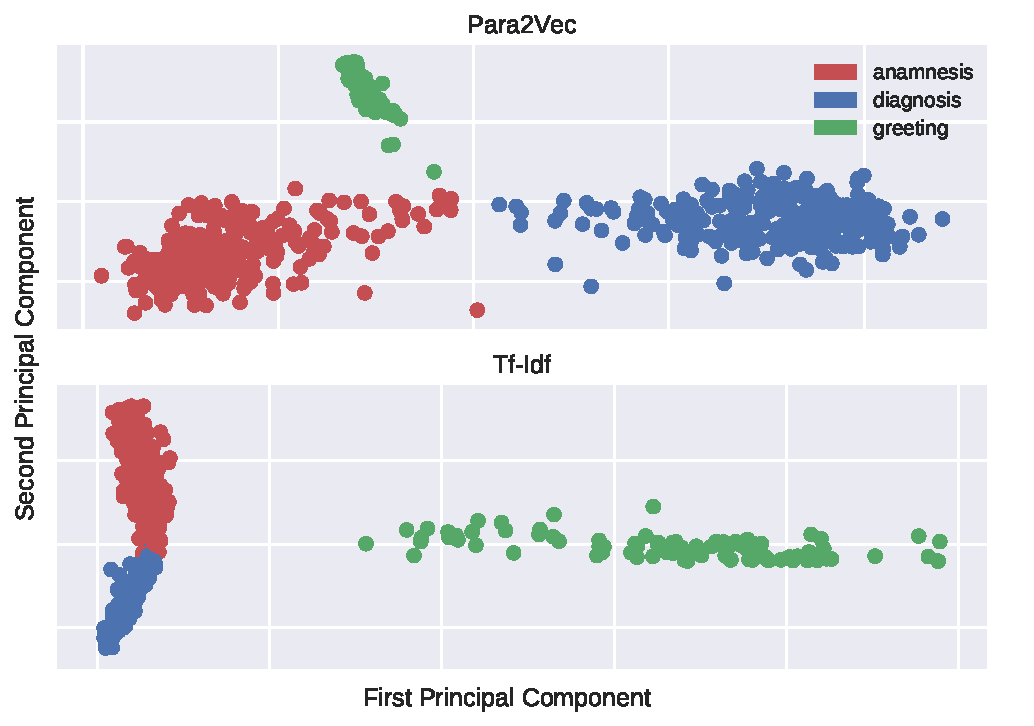
\includegraphics[width=\linewidth]{figures/para2vec_tfidf_pca}
	\caption{2D PCA projections of a vector space embedding of the physician letter paragraphs. Colors encode the respective paragraph category for each vector. \textbf{Top:} Paragraph vector space.  \textbf{Bottom:} Tf-idf vector space.}
	\label{fig:pv_tf_pca}
\end{figure}

\end{document}